%----------------------------------------------------------------------------
\appendix
%----------------------------------------------------------------------------
\chapter*{F�ggel�k}\addcontentsline{toc}{chapter}{F�ggel�k}
\setcounter{chapter}{6}  % a fofejezet-szamlalo az angol ABC 6. betuje (F) lesz
\setcounter{equation}{0} % a fofejezet-szamlalo az angol ABC 6. betuje (F) lesz
\numberwithin{equation}{section}
\numberwithin{figure}{section}
\numberwithin{lstlisting}{section}
%\numberwithin{tabular}{section}

%----------------------------------------------------------------------------
\section{A TeXnicCenter fel�lete}
%----------------------------------------------------------------------------
\begin{figure}[!ht]
\centering
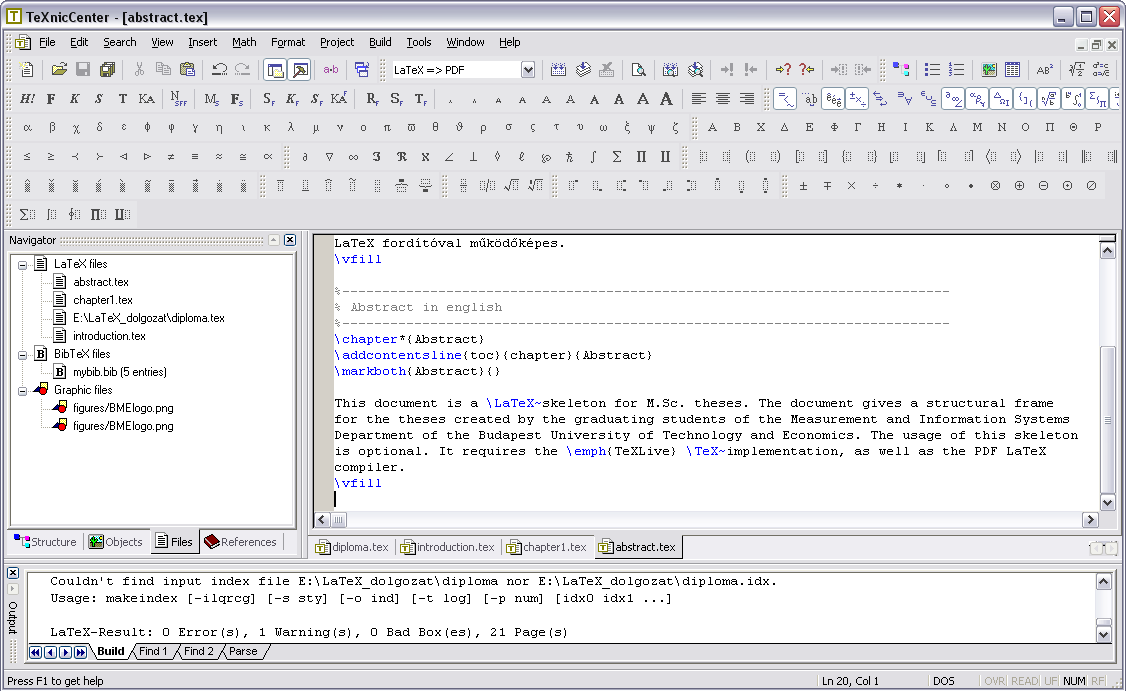
\includegraphics[width=150mm, keepaspectratio]{figures/TeXnicCenter.png}
\caption{A TeXnicCenter Windows alap� \LaTeX-szerkeszt�.} 
\end{figure}

%----------------------------------------------------------------------------
\clearpage\section{V�lasz az ,,�let, a vil�gmindens�g, meg minden'' k�rd�s�re}
%----------------------------------------------------------------------------
A Pitagorasz-t�telb�l levezetve
\begin{align}
c^2=a^2+b^2=42.
\end{align}
A Faraday-indukci�s t�rv�nyb�l levezetve
\begin{align}
\rot E=-\frac{dB}{dt}\hspace{1cm}\longrightarrow \hspace{1cm}
U_i=\oint\limits_\mathbf{L}{\mathbf{E}\mathbf{dl}}=-\frac{d}{dt}\int\limits_A{\mathbf{B}\mathbf{da}}=42.
\end{align}





